% ==============================================================================
% LAB 167
% MÄTNING PÅ ELEKTRISKA KRETSAR
% --------------------------
% Last updated <2015-03-10>
%
% Author:
% Jonas Sjöberg     <tel12jsg@student.hig.se>
% Oscar Wallberg    <tco13owg@student.hig.se>
%
% License:
% Creative Commons Attribution-NonCommercial-ShareAlike 4.0 International
% See LICENSE.md for full licensing information.
% ==============================================================================

% ==============================================================================
% INCLUDES AND CONFIGURATION
% ==============================================================================
\documentclass[11pt,a4paper]{article}
\usepackage[utf8]{inputenc}
\usepackage[swedish]{babel} % För svensk innehållsförteckning
\usepackage{siunitx} % (För dokumentation, kör i terminalen; texdoc siunitx)
\usepackage{amssymb}
\usepackage{amsmath}
\usepackage{amsfonts}
\usepackage{graphicx}
\usepackage{booktabs}
\usepackage{longtable} % Tables span across pages
\usepackage{microtype}
\usepackage{gensymb}
%\usepackage{tabto}
\usepackage{units}

\setlength\parindent{0pt} % Removes all indentation from paragraphs

% ==============================================================================
% DOCUMENT METADATA
% ==============================================================================
\title{EE466 \\ Lab 167 \\ Mätning på elektriska kretsar}

\author{\\
  Jonas Sjöberg\\
  Högskolan i Gävle,\\
  Elektronikingenjörsprogrammet,\\
  \texttt{tel12jsg@student.hig.se}\\
  \\
  Oscar Wallberg\\
  Högskolan i Gävle,\\
  Dataingenjörsprogrammet,\\
  \texttt{tco13owg@student.hig.se}\\}

\date{}
% ==============================================================================
\begin{document}
% ==============================================================================
\maketitle

\begin{center}
    \begin{tabular}{l r}
        Labb utförd: & 25 Februari 2015 \\
        Instruktör: & Efrain Zenteno
    \end{tabular}
\end{center}

% ==============================================================================
% ABSTRACT
% ==============================================================================
\begin{abstract}
    Syftet med laborationen är att praktiskt pröva några av de grundläggande
    sambanden och satserna i likströmsläran, samt att förstå enkla
    växelströmskretsar. Dessutom bör studenten efter genomförd laboration
    översiktligt förstå universalinstrumentets och oscilloskopets principiella
    funktionssätt, samt kunna tillämpa hanteringen av dessa instrument i
    mätning på elektriska kretsar.
\end{abstract}

\newpage

{
    %\hypersetup{linkcolor=black}
    \setcounter{tocdepth}{3}
    \tableofcontents
}

\newpage

% ==============================================================================
% SECTION: INTRODUKTION
% ==============================================================================
\section{Introduktion}\label{setup}
% ==============================================================================
% TODO: Allmän introduktion.


% ==============================================================================
% SECTION: 1 MÄTNING PÅ SERIESKRETS
% ==============================================================================
\section{Mätning på seriekrets}\label{}
% ==============================================================================
% TODO: Kopplingsschema.
Seriekretsen enligt figur \ref{fig:1-mm-schem} kopplades upp. 5 \si{\volt} valdes för spänningskällan.
\begin{figure}[htbp]
    \centering
        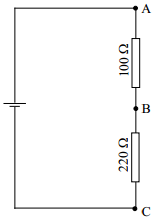
\includegraphics[scale=0.7]{misc/krets1.png}
    \caption{Seriekrets}
    \label{fig:1-mm-schem}
\end{figure}
\subsection{Mätresultat}\label{}
% ------------------------------------------------------------------------------
% TODO: + Spänningarna mellan AB, BC och AC.
Resistensen mellan A och B, $R_1$, mättes upp till $100.561 \ohm$ och mellan B och C, $R_2$, mättes $217.78 \ohm$ upp. Följande spänningar mättes därefter upp:
\begin{math}
U_{AB} = 1.58 \si{\volt}\\
U_{BC} = 3.41 \si{\volt}\\
U_{AC} = 4.999 \si{\volt}
\end{math}
\subsection{Kommentar}\label{}
% ------------------------------------------------------------------------------
% TODO: Kommentera utgående från Kirchhoffs 2:a lag.
%       Kommentera utgående från spänningsdelningslagen.
Spänningsdelningslagen ger:\\[+2mm]
\begin{math}
U_{AB} = U\times\frac{R_{1}}{R_{1}+R_{2}}\\[+2mm]
U_{AB} = 4.999\times\frac{100.561}{100.561+217.78}\\[+2mm]
U_{AB} = 1.579\\
\\
U_{BC} = U\times\frac{R_{2}}{R_{1}+R_{2}}\\[+2mm]
U_{BC} = 4.999\times\frac{217.78}{100.561+217.78}\\[+2mm]
U_{BC} = 3.42\\
\\
U_{AC} = U\times\frac{R_{1}+R_{2}}{R_{1}+R_{2}}\\[+2mm]
U_{AC} = U = 4.999\\
\end{math}

Kirchhoff's 2:a lag:
\begin{quote}
Summan av samtliga emk:s som ingår i en sluten krets är lika med summan av potentialfallen, eller\\
\begin{math}
u_{1} + u_{2} + \ldots + u_{n} = 0\\
\text{där }u_{k} \text{ betecknar en potentialändring.}
\end{math}
\end{quote}

Enligt Kirchhoff's lag:\\
$U - U_{AB} - U_{BC} = 0$\\
$4.99 - 1.579 - 3.42 = 0$, vilket stämmer.
% ==============================================================================
% SECTION: 2 iNVERKAN AV EN PARALLELLGREN PÅ EN KRETS
% ==============================================================================
\section{Inverkan av en parallellgren på en krets}\label{}
% ==============================================================================
% TODO: Kopplingsschema.
Ytterligare en resistor på 330 \si{\ohm} kopplades parallellt till kretsen från
figur \ref{fig:1-mm-schem}, se figur \ref{fig:2-mm-schem}.

\begin{figure}[htbp]
    \centering
        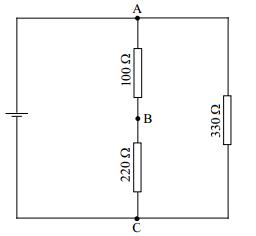
\includegraphics[scale=1.0]{misc/krets2.png}
    \caption{Parallellgren på föregående krets.}
    \label{fig:2-mm-schem}
\end{figure}
\subsection{Mätresultat}\label{}
% ------------------------------------------------------------------------------
% TODO: Mät strömmen i punkten B samt strömmen direkt från spänningskällan.
Strömmen som mättes vid spänningskällan var $33 \si{\milli\ampere}$ och strömmen i punkt B var $15.466 \si{\milli\ampere}$.
% ==============================================================================
% SECTION: 3 MÄTNING PÅ PARALLELLKRETS
% ==============================================================================
\section{Mätning på parallellkrets}\label{}
% ==============================================================================
% TODO: Kopplingsschema.
Två resistorer kopplades enligt figur \ref{fig:3-mm-schem}.
Sedan valdes 5 \si{\volt} för spänningskällan.

\begin{figure}[htbp]
    \centering
        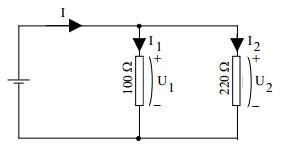
\includegraphics[scale=1]{misc/krets3.png}
    \caption{Parallellgren på föregående krets.}
    \label{fig:3-mm-schem}
\end{figure}
\subsection{Mätresultat}\label{}
% ------------------------------------------------------------------------------
% TODO: Mät de markerade strömmarna
$I_{1} = 47.35 \si{\milli\ampere}\\
I_{2} = 22.453 \si{\milli\ampere}\\
I = 72\si{\milli\ampere}$
\subsection{Kommentar}\label{}
% ------------------------------------------------------------------------------
% TODO: Kommentera utgående från Kirchhoffs 1:a lag.
Kirchhoff's 1:a lag:
\begin{quote}
Summan av alla elektriska strömmar som flyter till en nod är lika med summan av alla strömmar som flyter från noden, eller\\
$i_1 + i_2 \ldots + i_n = 0$\\
där $i_k$ betecknar en nodström.
\end{quote}
Detta ger\\
$I = I_{1} + I_{2}\\
I = 47.35 + 22.453 = 69.803\si{\milli\ampere}$\\
vilket ger en procentuell felmarginal på $\frac{72-69.803}{69.803}\times 100 = 3.147 \%$.
% ==============================================================================
% SECTION: 4 MÄTNING AV RESISTANS
% ==============================================================================
\section{Mätning av resistans}\label{}
% ==============================================================================
% TODO: Kopplingsschema.
Kretsarna funna i figur \ref{fig:4-mm-schem} kopplades upp. De uppmätta resistanserna var följande:\\
$R_{1} = 154.4\ohm\\
R_{2} = 177.75\ohm\\
R_{3} = 328\ohm\\
R_{4} = 118.3\ohm\\
R_{5} = 99.9\ohm$

\begin{figure}[htbp]
    \centering
        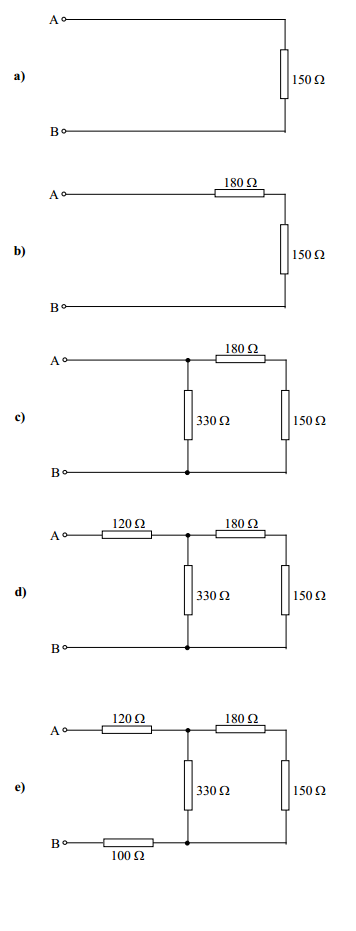
\includegraphics[scale=0.7]{misc/krets4.png}
    \caption{Resistorkretsar.}
    \label{fig:4-mm-schem}
\end{figure}
\subsection{Mätresultat}\label{}
% ------------------------------------------------------------------------------
% TODO: Mät resistansen mellan A och B i nedanstående kretsar.
\subsubsection{A}
$154.4 \ohm$
\subsubsection{B}
$331.7 \ohm$
\subsubsection{C}
$164.62 \ohm$
\subsubsection{D}
$283.52 \ohm$
\subsubsection{E}
$383.92 \ohm$
\subsection{Teoretisk beräkning}\label{}
% ------------------------------------------------------------------------------
% TODO: För varje mätning skall du verifiera resultatet med en teoretisk beräkning.
\subsubsection{A}
Resistansen $R_A$ i A utgörs av ett enda motstånd och kan utläsas
direkt till $R_{A} = R_{1} = $\unit[154.4]{\ohm}

\subsubsection{B}
Resistansen $R_{B}$ i B är teoretiskt;
% 180+150 = 330
\begin{align*}
R_{B}    &= R_{1} + R_{2}                        \\
         &= \unit[154.4]{\ohm} + \unit[177.75]{\ohm}  \\
         &= \unit[332.15]{\ohm}                     \\
\end{align*}

\subsubsection{C}
Resistansen $R_{C}$ i C är teoretiskt;
% 1/((1/330)+(1/(180+150))) = 165
\begin{align*}
R_{C}   &= \frac{1}{\frac{1}{R_{3}} + \frac{1}{R_{1} + R_{2}}} \\
        &= \frac{1}{\frac{1}{328\unit{\ohm}} + \frac{1}{\unit[154.4]{\ohm} + \unit[177.75]{\ohm}}} \\
        &= \unit[165.03]{\ohm}
\end{align*}

\subsubsection{D}
Resistansen $R_{D}$ i D är teoretiskt;
% 1/((1/330)+(1/(180+150)))+120 = 285
\begin{align*}
R_{D}   &= \frac{1}{\frac{1}{R_{3}} + \frac{1}{R_{1} + R_{2}}} + R_{4} \\
&= \frac{1}{\frac{1}{328\unit{\ohm}} + \frac{1}{\unit[154.4]{\ohm} + \unit[177.75]{\ohm}}} + \unit[118.3]{\ohm} \\
&= \unit[283.33]{\ohm}
\end{align*}

\subsubsection{E}
Resistansen $R_{E}$ i E är teoretiskt;
% 1/((1/330)+(1/(180+150)))+120+100 = 385
\begin{align*}
R_{E}   &= \frac{1}{\frac{1}{R_{3}} + \frac{1}{R_{1} + R_{2}}} + R_{4} + R_{5} \\
&= \frac{1}{\frac{1}{328\unit{\ohm}} + \frac{1}{\unit[154.4]{\ohm} + \unit[177.75]{\ohm}}} + \unit[118.3]{\ohm} + \unit[99.9]{\ohm}\\
&= \unit[383.23]{\ohm}
\end{align*}
\subsection{Kommentar}\label{}
% ------------------------------------------------------------------------------
% TODO: Kommentar på skillnader mellan mätresultat och beräkning?
Följande formel används för att beräkna den procentuella felmarginalen: \\[2mm]
%|teoretisk-uppmätt|/uppmätt * 100
$\frac{|\text{teoretiskt värde - uppmätt värde}|}{\text{uppmätt värde}}\times 100$
\subsubsection{A}
Den teoretiska beräkningen och den uppmätta stämmer överens; 154.4 \ohm.
\subsubsection{B}
$\frac{|332.15 - 331.7|}{331.7}\times 100 = 0.136\%$
\subsubsection{C}
$\frac{|165.03 - 164.62|}{164.62}\times 100 = 0.231\%$
\subsubsection{D}
$\frac{|283.33 - 283.52|}{283.52}\times 100 = 0.067\%$
\subsubsection{E}
$\frac{|383.23 - 383.92|}{383.92}\times 100 = 0.18\%$
% ==============================================================================
% SECTION: 5 MÄTNING AV EMK OCH INRE RESISTANS I EN TVÅPOL
% ==============================================================================
\section{Mätning av emk och inre resistans i en tvåpol}\label{measure_emk}
% ==============================================================================

\subsection{Mätning}
% ------------------------------------------------------------------------------
Dessa mätningar görs i syfte att undersöka konceptet tvåpol och demonstrera
konceptet av att studera och räkna med reducering av komplexa nät med hjälp av
Thévenins ekvivalens.
\par En så kallad experimentplatta eller "breadboard"
används för att konstruera kretsen som illustreras i Figur \ref{fig:5-schem}.
Nätaggregatet $V_{1}$ är ett strömbegränsande laboratorieaggregat HP3631A.
Spänningen $U$ mäts över dekadresistorn $R_{3}$ med bänkmultimetern $M_{2}$, en
HP34401A.  Strömmen $I$ mäts genom att den handhållna multimetern Tenma 72-2050
kopplas mellan punkten $A$ och $R_{3}$.
\par Källan som driver spänningen $V_{AB}$ utgörs av $V_{1}$, $R_{1}$ och $R_{2}$.
\par Lasten som är ansluten till utgången består av dekadresistorn $R_{3}$.
Resistansen hos multimetern $M_{2}$ parallellkopplas med $R_{3}$ och påverkar
således kretsen på ett oönskat sätt. Om man antar att $M_{2}$ har en inre
resistans på \unit[10]{\si{\Mohm}} förändras lastens effektiva resistans inte
märkbart, förutsatt att de uppmätta resistanserna är lågohmiga. Det förutsätts
såklart då också att kretsen ifråga inte är alltför känslig för
komponenttoleranser och yttre påverkan av till exempel mätinstrument.
\par Generellt kan antas att förändringen är försumbar då $R_{3}$ har ett lågt
värde men felvärdet blir klart påtagligt för högre värden av $R_{3}$.  Felvärdet
kan beräknas med Ekvation \ref{eq:err1} som vid en högre resistans enligt
\ref{eq:err2} blir 0,09\%, vilket är ett signifikant mätfel. 
Men eftersom att den maximala resistansen som används i det här fallet är
\unit[100]{\si{\kohm}} och felvärdet enligt Ekvation \ref{eq:err3} då blir
$\approx$ 0,0099\% kan belastningen från multimetern förbises.

\par Mätning på kopplingen ger att spänningen vid tvåpolens "utgång"
$V_{AB}$ = \unit[7.16]{\si{\volt}}.
\par Med $R_{3}$ ställd på sin maximala resistans är spänningen oförändrad.
När värdet hos $R_{3}$ sänks börjar spänningen vid tvåpolens utgång också att
sjunka.
\par Halva tomgångsspänningen $\frac{V_{AB}}{2} = \unit[3.58]{\si{\volt}}$
avläses vid en last av $R_{3}$ = \unit[341]{\si{\ohm}}.  Strömmen genom lasten
är då $I = \unit[10.531]{\si{\mA}}$.

% fel(%) = [(uppmätt - förväntat) / förväntat] * 100
% (((1/((1/x)+(1/(10e6))))-x)/x)*100
\begin{equation}\label{eq:err1}
\text{Felvärde}(\si{\percent}) =
\frac{\text{Uppmätt värde} - \text{Förväntat värde}}{\text{Förväntat värde}} \times 100
\end{equation}

\begin{align}
\text{Felvärde }{R}_{last}(\si{\percent}) &= \frac{(\frac{1}{\frac{1}{R_{3}}+\frac{1}{R{M_{2}}}}) - R_{3}}{R_{3}} \times 100 \label{eq:err2}\\
&= \frac{(\frac{1}{\frac{1}{\unit[1]{\si{\Mohm}}}+\frac{1}{\unit[10]{\si{\Mohm}}}}) - \unit[1]{\si{\Mohm}}}{\unit[1]{\si{\Mohm}}} \times 100\\
&= 0,09 \%
\end{align}

\begin{align}
\text{Felvärde }{R}_{last}(\si{\percent}) &= \frac{(\frac{1}{\frac{1}{R_{3}}+\frac{1}{R{M_{2}}}}) - R_{3}}{R_{3}} \times 100 \label{eq:err3}\\
&= \frac{(\frac{1}{\frac{1}{\unit[100]{\si{\kohm}}}+\frac{1}{\unit[10]{\si{\Mohm}}}}) - \unit[1]{\si{\Mohm}}}{\unit[100]{\si{\kohm}}} \times 100\\
&= 0,009901 \%
\end{align}

\begin{figure}
\centering
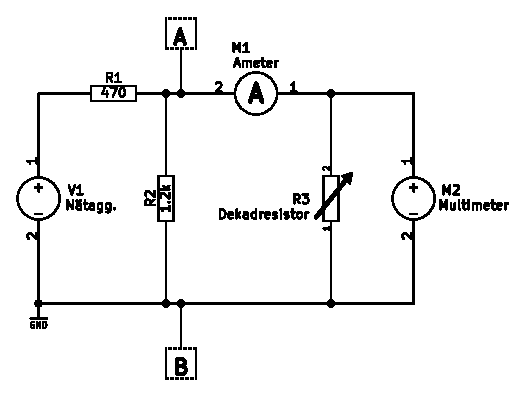
\includegraphics[width=0.7\linewidth]{img/5-schem}
\caption[Kopplingsschema för mätning av tvåpol.]
{Koppling vid mätning av EMK och inre resistans i en tvåpol.}
\label{fig:5-schem}
\end{figure}


\subsection{Teoretisk härledning med Thévenins teorem}
% ------------------------------------------------------------------------------
Kretsen som levererar spänningen ritas om till den i Figur
\ref{fig:5-thevenin-schem}.

\begin{figure}
    \centering
    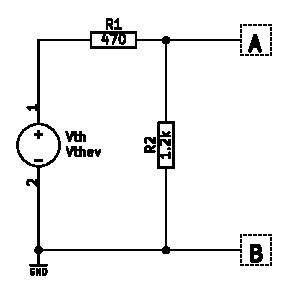
\includegraphics[width=0.4\linewidth]{img/5-thevenin-schem}
    \caption[Théveninekvivalens]
    {Den obelastade kretsen som utgör källpolspänningen}
    \label{fig:5-thevenin-schem}
\end{figure}

Den obelastade "tomgångsspänningen" mellan punkterna A och B, $V_{AB}$ beräknas
enligt Ekv. \ref{eq:thev1}.
% 10*(1,2e3/(470+1,2e3)) = 7,18562874251497005988
\begin{equation}\label{eq:thev1}
\begin{split}
V_{AB} = V_{th} \times \frac{R_2}{R_1 + R_2}\\
V_{AB} = \unit[10]{\si{\volt}} \times \frac{\unit[1.2]{\si{\kohm}}}{\unit[470]{\si{\ohm}}+ \unit[1.2]{\si{\kohm}}}\\
V_{AB} = \unit[10]{\si{\volt}} \times \frac{\num{1.2e3}}{\num{470}+\num{1.2e3}}\\
V_{AB} = \unit[7,185]{\si{\volt}}
\end{split}
\end{equation}

Den inre resistansen beräknas genom att kortsluta spänningskällan.
Kretsen blir då den i Figur \ref{fig:5-thevenin-schem2}.

\begin{figure}
    \centering
    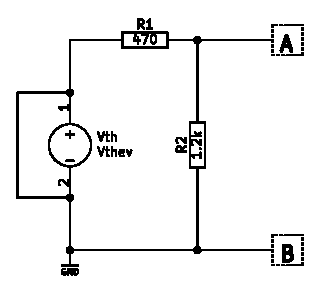
\includegraphics[width=0.4\linewidth]{img/5-thevenin-schem2}
    \caption[Beräkning av Théveninekvivalens]
    {Spänningskälla kortsluten för att hitta inre resistans}
    \label{fig:5-thevenin-schem2}
\end{figure}

Den inre resistansen utgörs av parallellkopplingen $R_{1}$ och $R_{2}$ och
beräknas enligt Ekv. \ref{eq:thev2}.
% (470*1200)/(470+1200) = 337,72455089820359281437
\begin{equation}\label{eq:thev2}
\begin{split}
R_{th} = \frac{1}{\frac{1}{R_{1}} + \frac{1}{R_{2}}}\\
R_{th} = \frac{1}{\frac{1}{\unit[470]{\si{\ohm}}} + \frac{1}{\unit[1.2]{\si{\kohm}}}}\\
R_{th} = \unit[337,72]{\si{\ohm}}
\end{split}
\end{equation}

De teoretiska värdena för Théveninekvivalensen i \ref{eq:thev3} används i Figur
\ref{fig:5-thevenin-schem3} som har ett beteende ekvivalent med den
ursprungliga tvåpolen.

\begin{align}\label{eq:thev3}
V_{AB} &= \unit[7,185]{\si{\volt}}\\
R_{th} &= \unit[337,72]{\si{\ohm}}
\end{align}

\begin{figure}
    \centering
    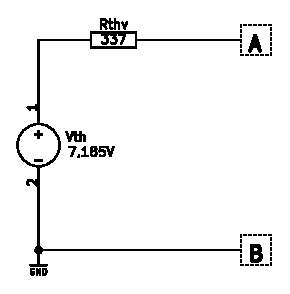
\includegraphics[width=0.4\linewidth]{img/5-thevenin-schem3}
    \caption[Beräkning av Théveninekvivalens]
    {Fullständig ekvivalent krets}
    \label{fig:5-thevenin-schem3}
\end{figure}


\subsection{Kommentar}
% ------------------------------------------------------------------------------
Att reducera kretsar eller hela apparater till en enkel svart låda med två
anslutningar vars funktion helt kan beskrivas med Thévenins teorem är en teknik
som används mycket ofta vid design och analys av kretsar.
Det gör det möjligt att bryta ner en större konstruktion till mindre moduler
som kan analyseras var för sig. Relevant för området är bestämning av
ingångsimpedans och utgångsimpedans, förmåga att driva andra kretsar eller 
apparater. Det är mycket viktigt att relativt enkelt kunna förutse hur olika
moduler eller sektioner skulle komma att påverkas av att kopplas samman.


% ==============================================================================
% SECTION: 6 KARAKTERISTIK HOS EN LYSDIOD
% ==============================================================================
\section{Karakteristik hos en lysdiod}\label{}
% ==============================================================================
För att undersöka \nicefrac{I}{V}-karakteristiken hos en lysdiod behövs kännedom
om spänningen över lysdioden, $V_{LED}$ samt strömmen genom lysdioden, $I_{LED}$.
\par Kretsen i Figur \ref{fig:6-schem} konstruerades på en kopplingsplatta.
En röd lysdiod användes, vi kan anta att det röda ljusets våglängd är cirka
\unit[660]{\si{\nm}} och därmed förvänta oss ett framspänningsfall på
cirka \unit[1.8]{\si{\volt}} vid \unit[20]{\si{\mA}}. Framspänningsfallet
$V_{f}$ brukar i datablad ofta specificeras vid \unit[20]{\si{\mA}}, som också
många gånger är lysdiodens rekommenderade maxström.
\par Resistorn $R_{2}$ förhindrar strömmen $I_{LED}$ att bli alldeles för stor
i det fall att resistansen hos dekadresistorn $R_{1}$ är ställd till ett
lågt värde eller direkt kortslutning. Den högsta ström som kan flyta genom 
kretsen uppskattas i Ekvation \ref{eq:ledmax} till ett värde under den 
specificerade maxgränsen på \unit[20]{\si{\mA}}.

% (10-1,8)/470 = 0,01744680851063829787
\begin{equation}\label{eq:ledmax}
\begin{split}
I_{LED_{max}} = \frac{V_{1} - V_{D1}}{R_{2}}\\
I_{LED_{max}} = \frac{\unit[10]{\si{\volt}} - \unit[1.8]{\si{\volt}}}{\unit[470]{\si{\ohm}}}\\
I_{LED_{max}} = \unit[17.4]{\si{\mA}}
\end{split}
\end{equation}

\par Lysdioden är precis som namnet antyder en typ av diod och uppvisar en
typisk diodkarakteristik, där strömmen $I_{diod}$ är näst intill obefintlig då
$V_{diod} < V_{f}$ för att sedan öka exponentiellt efter det att
$V_{diod} \ge V_{f}$ och dioden börjar leda.
Förhållandet mellan spänning och ström är olinjärt, $\Delta I$ är mycket stort
över ett mycket litet område av $\Delta V$.
\par Mätresultaten presenteras i Tabell \ref{6-table}, Figur 
\ref{fig:led-data-graf} och Figur \ref{fig:led-data-graf2} under sektion 
\ref{led-results}.

\begin{figure}
    \centering
    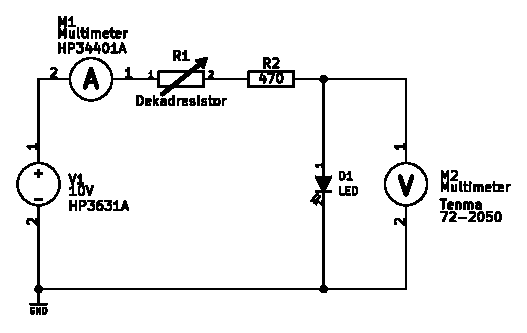
\includegraphics[width=0.8\linewidth]{img/6-schem}
    \caption[Bestämning av I/V-karakteristik hos LED]
    {Labbkoppling för att bestämma \nicefrac{I}{V}-karakteristik för en LED}
    \label{fig:6-schem}
\end{figure}


\subsection{Mätresultat}\label{led-results}
% ------------------------------------------------------------------------------

\begin{longtable}[c]{@{}ccc@{}}
    \toprule\addlinespace
    \begin{tabular}{ll}$R_{3}$
    \end{tabular} & \begin{tabular}{ll}$I_{LED}$
\end{tabular} & \begin{tabular}{ll}$V_{LED}$
\end{tabular}
\\\addlinespace
\midrule\endhead
\unit[500]{\si{\ohm}} & \unit[16.38]{\si{\unit{\mA}}} & \unit[1.78]{\si{\volt}}
\\\addlinespace
\unit[600]{\si{\ohm}} & \unit[13.66]{\si{\unit{\mA}}} & \unit[1.766]{\si{\volt}}
\\\addlinespace
\unit[700]{\si{\ohm}} & \unit[11.725]{\si{\unit{\mA}}} & \unit[1.755]{\si{\volt}}
\\\addlinespace
\unit[800]{\si{\ohm}} & \unit[10.269]{\si{\unit{\mA}}} & \unit[1.744]{\si{\volt}}
\\\addlinespace
\unit[900]{\si{\ohm}} & \unit[9.1342]{\si{\unit{\mA}}} & \unit[1.737]{\si{\volt}}
\\\addlinespace
\unit[1]{\si{\kohm}} & \unit[8.260]{\si{\unit{\mA}}} & \unit[1.730]{\si{\volt}}
\\\addlinespace
\unit[2]{\si{\kohm}} & \unit[3.3319]{\si{\unit{\mA}}} & \unit[1.685]{\si{\volt}}
\\\addlinespace
\unit[3]{\si{\kohm}} & \unit[2.3805]{\si{\unit{\mA}}} & \unit[1.671]{\si{\volt}}
\\\addlinespace
\unit[4]{\si{\kohm}} & \unit[1.8525]{\si{\unit{\mA}}} & \unit[1.662]{\si{\volt}}
\\\addlinespace
\unit[5]{\si{\kohm}} & \unit[1.5176]{\si{\unit{\mA}}} & \unit[1.655]{\si{\volt}}
\\\addlinespace
\unit[6]{\si{\kohm}} & \unit[1.2858]{\si{\unit{\mA}}} & \unit[1.648]{\si{\volt}}
\\\addlinespace
\unit[7]{\si{\kohm}} & \unit[1.1159]{\si{\unit{\mA}}} & \unit[1.643]{\si{\volt}}
\\\addlinespace
\unit[8]{\si{\kohm}} & \unit[985.6]{\si{\unit{\uA}}} & \unit[1.637]{\si{\volt}}
\\\addlinespace
\unit[9]{\si{\kohm}} & \unit[882.5]{\si{\unit{\uA}}} & \unit[1.6304]{\si{\volt}}
\\\addlinespace
\unit[10]{\si{\kohm}} & \unit[799.2]{\si{\unit{\uA}}} & \unit[1.630]{\si{\volt}}
\\\addlinespace
\unit[20]{\si{\kohm}} & \unit[408.7]{\si{\unit{\uA}}} & \unit[1.605]{\si{\volt}}
\\\addlinespace
\unit[30]{\si{\kohm}} & \unit[275.3]{\si{\unit{\uA}}} & \unit[1.590]{\si{\volt}}
\\\addlinespace
\unit[40]{\si{\kohm}} & \unit[2077]{\si{\unit{\uA}}} & \unit[1.578]{\si{\volt}}
\\\addlinespace
\unit[50]{\si{\kohm}} & \unit[1667]{\si{\unit{\uA}}} & \unit[1.569]{\si{\volt}}
\\\addlinespace
\unit[60]{\si{\kohm}} & \unit[139.2]{\si{\unit{\uA}}} & \unit[1.567]{\si{\volt}}
\\\addlinespace
\unit[70]{\si{\kohm}} & \unit[496.]{\si{\unit{\uA}}} & \unit[1.556]{\si{\volt}}
\\\addlinespace
\unit[80]{\si{\kohm}} & \unit[104.8]{\si{\unit{\uA}}} & \unit[1.55]{\si{\volt}}
\\\addlinespace
\unit[90]{\si{\kohm}} & \unit[93.3]{\si{\unit{\uA}}} & \unit[1.545]{\si{\volt}}
\\\addlinespace
\unit[100]{\si{\kohm}} & \unit[84.0]{\si{\unit{\uA}}} & \unit[1.541]{\si{\volt}}
\\\addlinespace
\bottomrule
\addlinespace
\caption[]{Mätresultat för kretsen i Figur \ref{fig:5-schem}.}
\label{6-table}
\end{longtable}

\begin{figure}
    \centering
    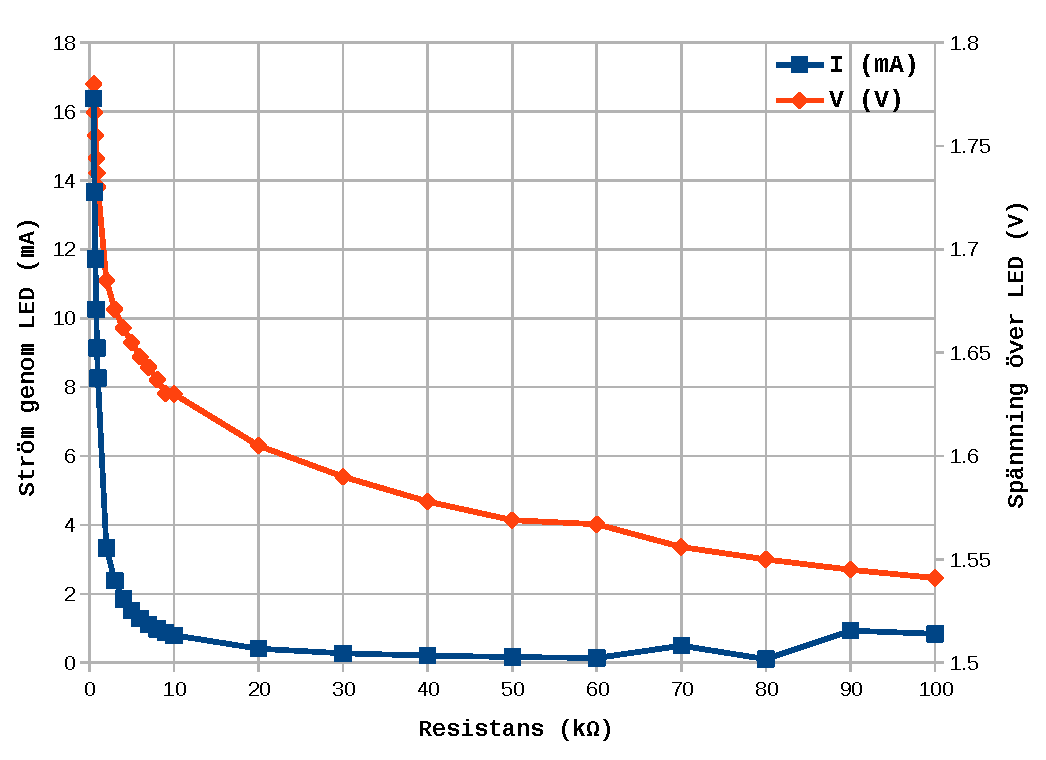
\includegraphics[width=\linewidth]{img/6-led_data-graf}
    \caption[Spänning och ström genom LED som funktion av serieresistans]
    {Ström genom och spänning över LED som en funktion av resistans}
    \label{fig:led-data-graf}
\end{figure}

\begin{figure}
    \centering
    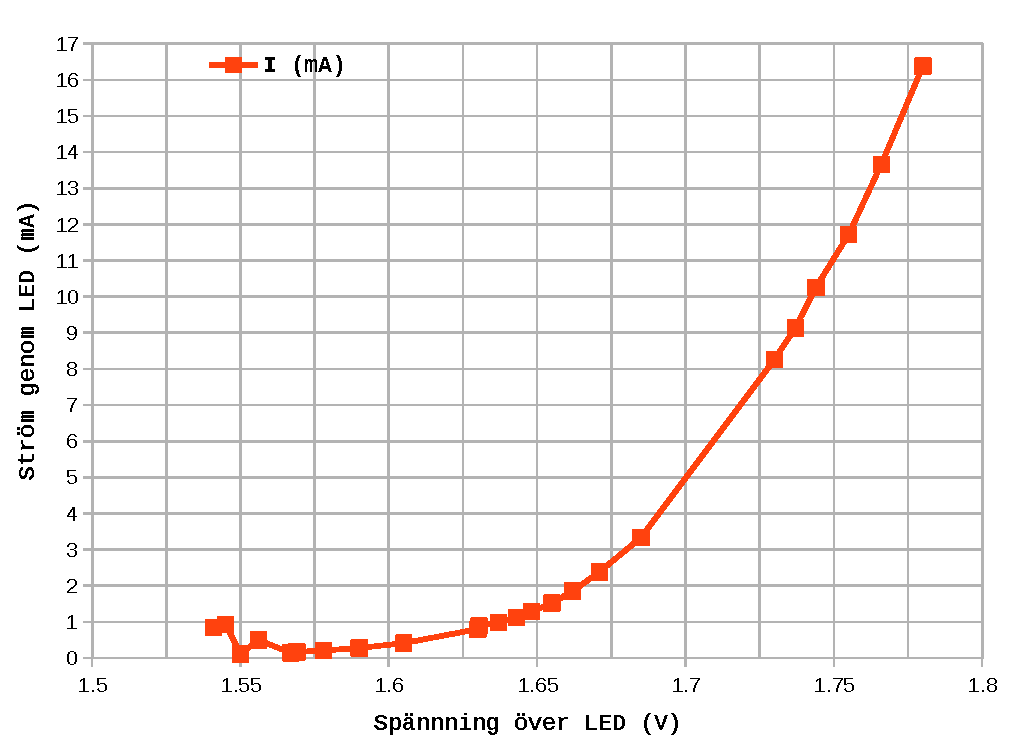
\includegraphics[width=\linewidth]{img/6-led_data-graf2}
    \caption[Ström genom LED som funktion av spänning över LED]
    {Ström genom LED som en funktion av spänning över LED}
    \label{fig:led-data-graf2}
\end{figure}


\subsection{Kommentar}
% ------------------------------------------------------------------------------
Mätningarna stämmer överens med antagandet att lysdiodens framspänningsfall
$V_{f}$ är omkring \unit[1.8]{\si{\volt}} då $I_{LED} \approx \unit[20]{\si{\mA}}$.
\par Lysdioder drivs som lämpligast med en låg spänning och en hög ström, ofta
används kretsar som levererar en konstant ström, \emph{constant current source}.
till exempel kretsen i Figur \ref som är en spänningsstyrd strömgenerator, som driver
flera lysdioder med samma ström, med ett linjärt förhållande mellan styrspänning
och diodström. Kretsen användes för att besvara en förfrågan om hur flera LEDs
kan drivas med samma ström under en enkel $+9V$ spänningsmatning.

\begin{figure}
    \centering
    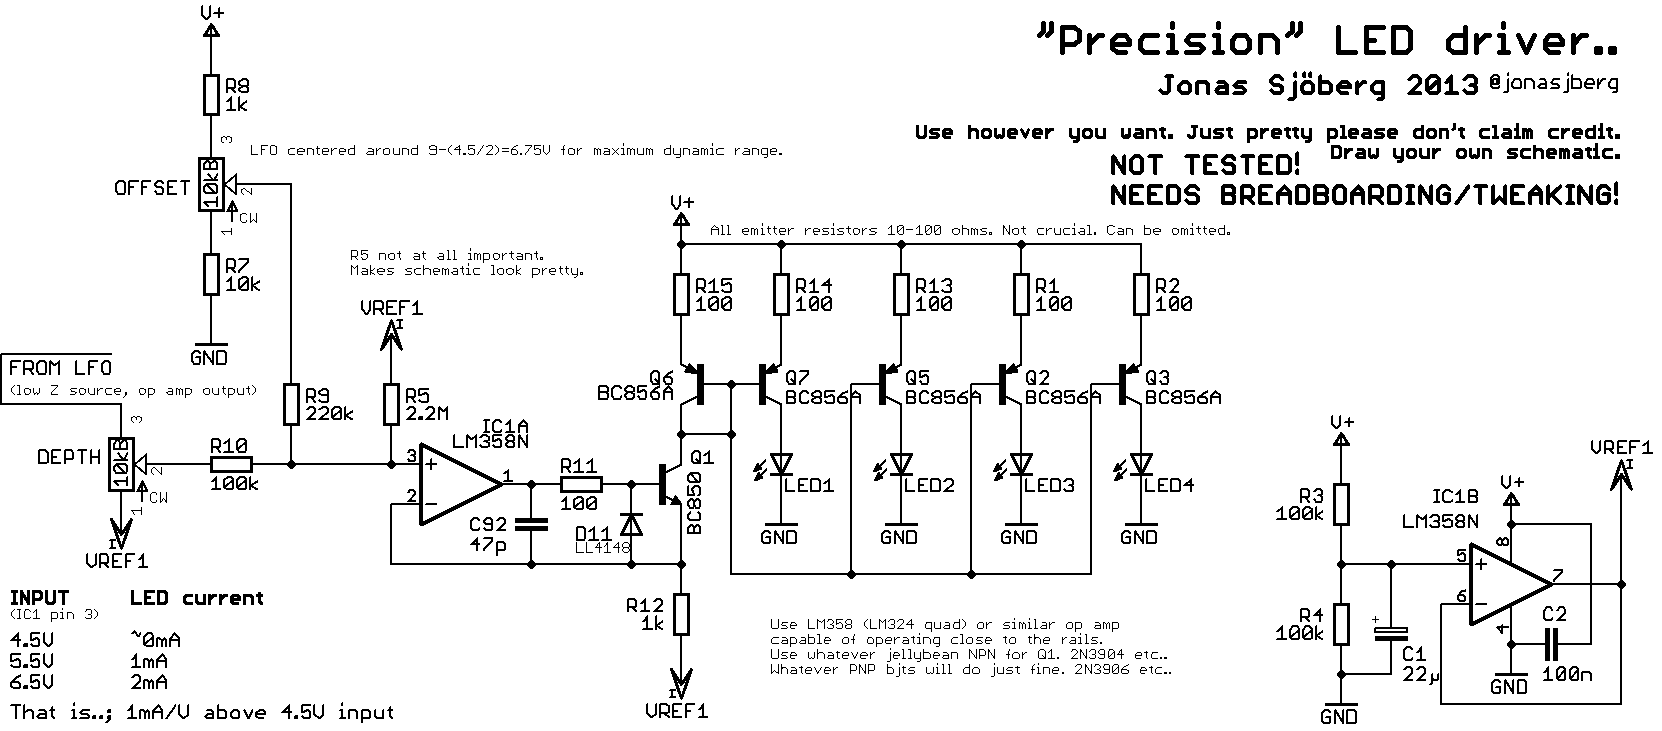
\includegraphics[width=\linewidth]{img/LED-driver}
    \caption[Spänningsstyrd LED-drivare för osymmetrisk spänningsmatning]
    {Exempel på spänningsstyrd LED-drivare för osymmetrisk spänningsmatning}
    \label{fig:led-data-graf2}
\end{figure}


% ==============================================================================
% SECTION: 7 MÄTNING AV VÄXELSPÄNNING MED UNIVERSALINSTRUMENT OCH OSCILLOSKOP
% ==============================================================================
\section{Mätning av växelspänning med universalinstrument och oscilloskop}
% ==============================================================================
För att generera en växelspänning används signalgeneratorn HP33120A, vars
utgång kopplas till en BNC T-koppling, som förgrenar signalen till både
multimetern HP34401A och oscilloskopet. En adapter används för att ansluta BNC
T-kopplingen till vanliga "banan" labsladdar som kopplas till multimetern. Se
Figur \ref{fig:foto1} och Figur \ref{fig:foto2}.
\par Signalgeneratorn konfigureras för att generera en sinusformad signal med
en frekvens på \unit[1]{\si{\kHz}} och en amplitud på $\nicefrac{V_{pp}}{2}$.
Signalgeneratorn anger amplitud som halva topp-till-topp-värdet.
\par Multimetern ställs för att mäta $V_{AC}$ RMS med
automatisk inställning av mätområde. På oscilloskopet används funktioner under
\emph{measure} för att direkt visa signalens amplitud i $V_{pp}$. Oscilloskopet
visar signalens amplitud från topp-till-topp, det vill säga dubbla det hos
signalgeneratorn.

\begin{figure}
    \centering
    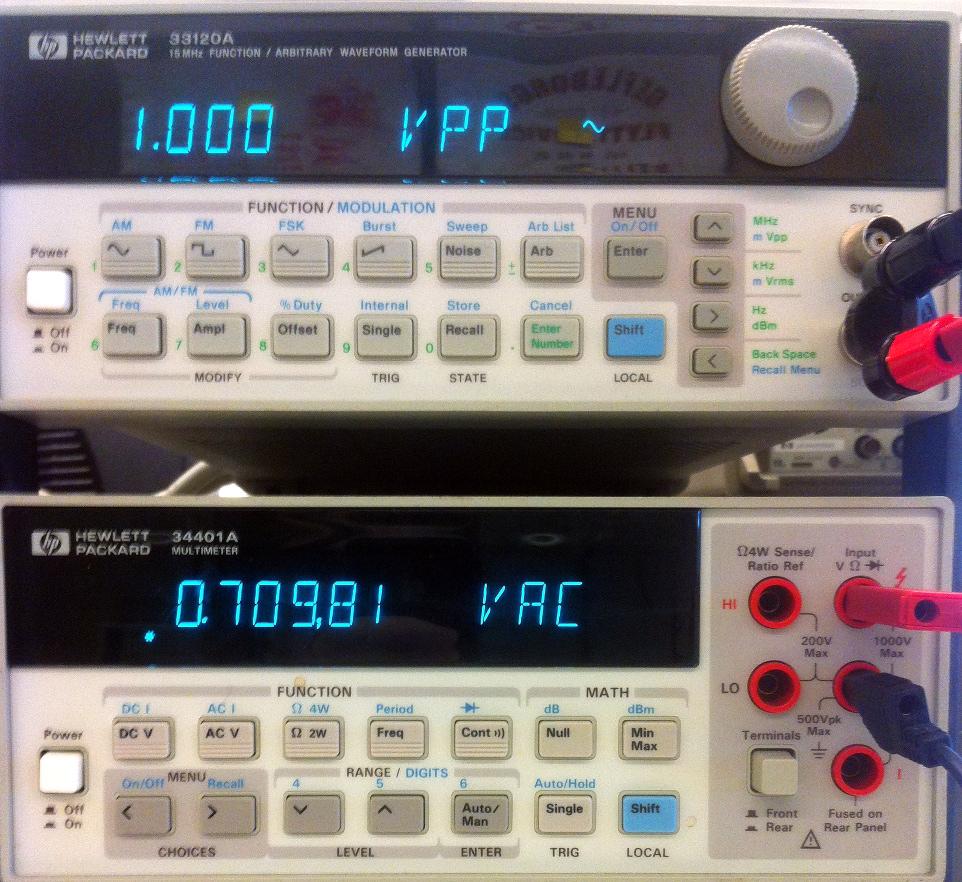
\includegraphics[width=\linewidth]{img/foto1}
    \caption[]
    {Multimeter och signalgenerator under mätning}
    \label{fig:foto1}
\end{figure}

\begin{figure}
    \centering
    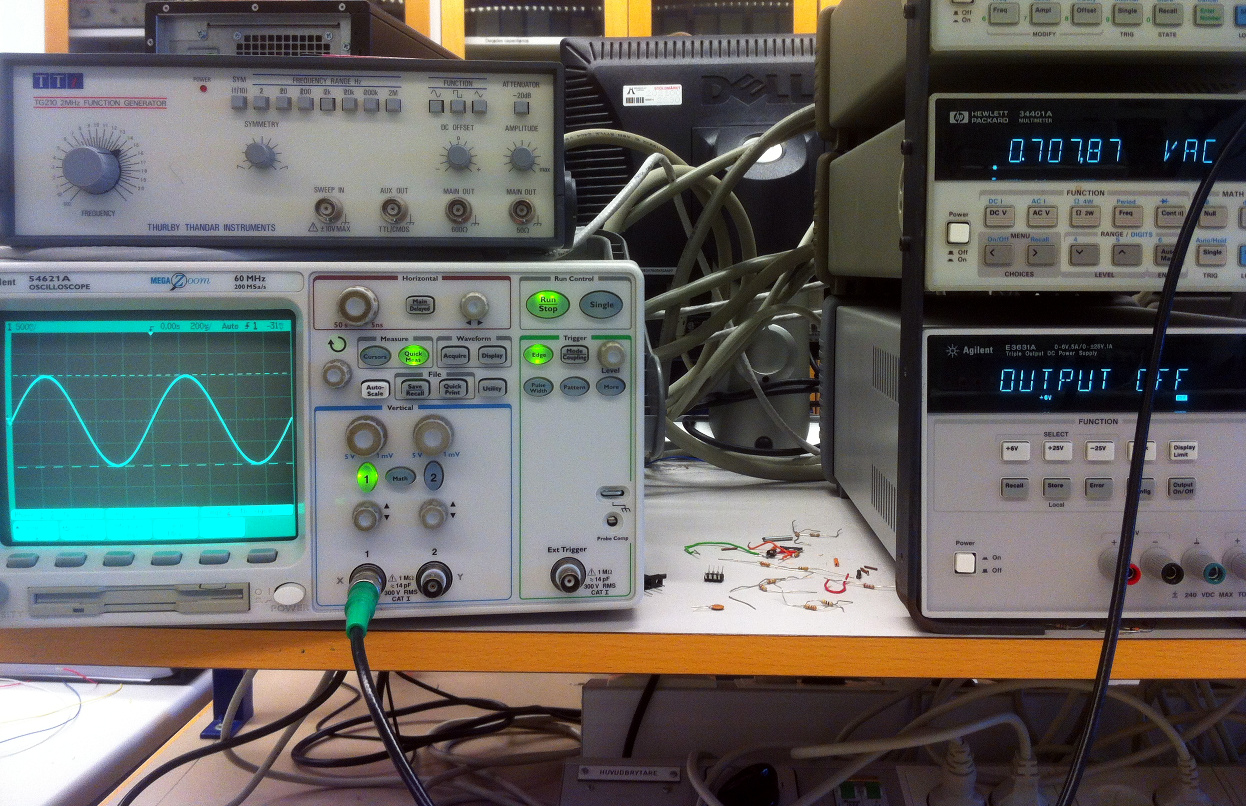
\includegraphics[width=\linewidth]{img/foto2}
    \caption[]
    {Multimeter och signalgenerator under mätning}
    \label{fig:foto2}
\end{figure}


\subsection{Mätresultat}\label{}
% ------------------------------------------------------------------------------
Förhållandet mellan  $V_{AC}$ RMS och $V_{pp}$ kan skrivas som i Ekvation
\ref{eq:rms-eq}.

\begin{equation}\label{eq:rms-eq}
\begin{split}
V_{AC} RMS = \frac{V_{pp}}{2} \times \frac{1}{\sqrt{2}}\\
\end{split}
\end{equation}

% 1/sqrt(2) = 0,7071067811865475244
Anmärkningsvärt är förhållandet mellan de tre storheterna, $\nicefrac{V_{pp}}{2}$,
$V_{AC}$ RMS och $V_{pp}$ i Ekvation \ref{eq:rms-eq2}. RMS-värdet förhåller sig
till peak-värdet med en ratio av $\frac{1}{\sqrt{2}} \approx 0.707106 \ldots$

\begin{align}\label{eq:rms-eq2}
%\begin{split}
\nicefrac{V_{pp}}{2} &= \frac{V_{pp}}{2}\\
V_{AC}\text{ RMS} &= \frac{V_{pp}}{2} \times \frac{1}{\sqrt{2}}\\
V_{pp} &= 2 \times (\nicefrac{V_{pp}}{2})
%\end{split}
\end{align}

Signalens frekvens utläses direkt på oscilloskopskärmen. Den kan annars lätt
härledas från sambandet $f = \frac{1}{T}$, där perioden $T$ kan utläsas direkt
genom att uppskatta signalens storlek till skärmens rutnät och multiplicera med
\nicefrac{tid}{div}, det vill säga värdet varje ruta motsvarar. För en sinusformad
signal är det lämpligt att mäta periodtiden mellan två nollgenomgångspunkter och
därefter omvandla från period till frekvens.
\par Om en signal upprepas inom två divisioner och \nicefrac{tid}{div} är ställd
på \nicefrac{\unit[500]{\si{\us}}}{div}, fås en periodtid \unit[1]{\si{\ms}}
och frekvensen kan beräknas $f = \frac{1}{\num{1e-3}} = \unit[1]{\si{\kHz}}$.

\subsection{Kommentar}
% ------------------------------------------------------------------------------
Oscilloskopet visar sannolikt det noggrannaste värdet för signalens frekvens.
Däremot är multimetern troligtvis noggrannare vid mätning av RMS-värde.
Den använda multimetern HP34401A har så kallad \emph{true RMS}-funktionalitet
vilket möjliggör mätning av signaler av signaler med godtycklig vågform. Den är
därför med största sannolikhet det mest precisa instrumentet för att mäta RMS
i experimentet.
\par I enklare multimeters uppskattas ofta RMS-värdet genom att den uppmätta
signalen antas vara sinusformad och omvandlingen sker med helvågslikriktning,
toppvärdesdetektion och multiplikation med konstanten $\frac{1}{\sqrt{2}}$.
\par Vi kan vara relativt säkra på att den frekvens och amplitud som ställs in
på signalgeneratorn är den som faktiskt finns vid signalgeneratorns utgång,
detta till följd av att signalgeneratorn är digital och genererar signalerna
med en DAC. En analog signalgenerator uppvisar en stor intolerans för
temperaturförändringar och många av komponenters icke-ideala egenskaper
påverkar stabilitet och precision.  Kalibrering är mycket viktigare för ett
analogt instrument. Det digitala instrumentets analoga signalväg, från
D/A-omvandlaren genom en drivförstärkare till utgången, är förhållandevis kort
och några eventuella fel kan kalibreras bort genom kompensationer i mjukvaran.

\pagebreak

\begin{longtable}[c]{@{}cccc@{}}
    \toprule\addlinespace
    \begin{tabular}{ll}Inställd\\vågform
    \end{tabular} & \begin{tabular}{ll}Inställd\\amplitud\\($\nicefrac{V_{pp}}{2}$)
\end{tabular} & \begin{tabular}{ll}Uppmätt med\\multimeter\\($V_{AC}$ RMS)
\end{tabular} & \begin{tabular}{ll}Uppmätt med\\oscilloskop\\($V_{pp}$)
\end{tabular}
\\\addlinespace
\midrule\endhead
Sinus & 1 & 0.7081 & 2.06
\\\addlinespace
      & 2 & 1.4149 & 4.13
\\\addlinespace
      & 3 & 2.1253 & 6.06
\\\addlinespace
      & 4 & 2.8324 & 8.19
\\\addlinespace
      & 5 & 3.5421 & 10.13
\\\addlinespace
\midrule
Fyrkant & 1 & 1.00095 & 2.02
\\\addlinespace
        & 2 & 2.0006  & 4.07
\\\addlinespace
        & 3 & 3.004   & 6.07
\\\addlinespace
        & 4 & 4.0042  & 8.07
\\\addlinespace
        & 5 & 5.0038  & 10.07
\\\addlinespace
\midrule
Triangel & 1 & 0.5779 & 2.13
\\\addlinespace
         & 2 & 1.1555 & 4.13                
\\\addlinespace
         & 3 & 1.7335 & 6.13                    
\\\addlinespace
         & 4 & 2.3122 & 8.13                
\\\addlinespace
         & 5 & 2.8922 & 10.13                   
\\\addlinespace
\midrule
Ramp     & 1 & 0.5778 &  2.11               
\\\addlinespace
         & 2 & 1.1552 &  4.22                   
\\\addlinespace
         & 3 & 1.7332 &  6.25               
\\\addlinespace
         & 4 & 2.3118 &  8.38                    
\\\addlinespace
         & 5 & 2.8918 &  10.44              
\\\addlinespace
\bottomrule
\addlinespace
\caption{Mätresultat för mätning av växelspänning med universalinstrument och
    oscilloskop.}
\label{vdivtable1}
\end{longtable}

% ==============================================================================
% SECTION: 8 STUDIUM AV FREKVENSGÅNG I EN REAKTIV KRETS
% ==============================================================================
\section{Studium av frekvensgång i en reaktiv krets}\label{}
% ==============================================================================
% TODO: Kopplingsschema.
Kretsen funnen i figur \ref{fig:8-schem} kopplades upp.
\begin{figure}[htbp]
    \centering
        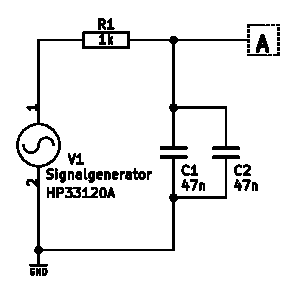
\includegraphics[scale=1.0]{img/8-schem.eps}
    \caption{Reaktiv krets.}
    \label{fig:8-schem}
\end{figure}
\subsection{Mätresultat}\label{}
% ------------------------------------------------------------------------------
% TODO: + Gör upp en tabell som för varje frekvens anger
%         - tongeneratorns signalamplitud,
%         - amplituden hos spänningen över den studerade kondensatorn
%         - kvoten mellan den senare amplituden och den tidigare
%         - samt om fasförskjutning förekommer.
Frekvensen varierades mellan 100 \si{\hertz} och 1900 \si{\hertz} i steg om 200 \si{\hertz} med en konstant spänning på tongeneratorn; $2.09\si{\volt}$. Tabell \ref{8a-table} presenterar resultatet.
\begin{longtable}[c]{@{}ccccc@{}}
    \toprule\addlinespace
    \begin{tabular}{ll}$Frekvens, \si{\hertz}$
    \end{tabular} & \begin{tabular}{ll}$Kondensator, \si{\volt}$
\end{tabular} & \begin{tabular}{ll}$\frac{u_{c}}{u_{TG}}$
\end{tabular} & \begin{tabular}{ll}$\text{Fasförskjutning}, \celsius$
\end{tabular}
\\\addlinespace
\midrule\endhead
100 & 2.11 & 1.01 & 5
\\\addlinespace
300 & 2.06 & 0.99 & 10
\\\addlinespace
500 & 2 & 0.96 & 17
\\\addlinespace
700 & 1.94 & 0.93 & 24
\\\addlinespace
900 & 1.84 & 0.88 & 29
\\\addlinespace
1100 & 1.75 & 0.84 & 33
\\\addlinespace
1300 & 1.66 & 0.79 & 37
\\\addlinespace
1500 & 1.56 & 0.75 & 42
\\\addlinespace
1700 & 1.49 & 0.71 & 45
\\\addlinespace
1900 & 1.39 & 0.67 & 49
\\\addlinespace
\bottomrule
\addlinespace
\caption[]{Mätresultat för kretsen i Figur \ref{fig:8-schem}.}
\label{8a-table}
\end{longtable}
\subsection{Teoretisk beräkning}\label{}
% ------------------------------------------------------------------------------
% TODO: Kontrollera dina resultat genom att utnyttja följande formel: 
Följande formel används för att teoretiskt beräkna kvoten mellan kondensatorns spänning och tongeneratorns:\\[2mm]
$\frac{u_{c}}{u_{TG}} = \frac{1}{\sqrt{1+(2 \pi \times f \times R \times C)^2}}$\\[2mm]
Det teoretiska resultatet redovisas i tabell \ref{8b-table}.
\begin{longtable}[c]{@{}cc@{}}
    \toprule\addlinespace
    \begin{tabular}{ll}$Frekvens, \si{\hertz}$
    \end{tabular} & \begin{tabular}{ll}$\frac{u_{c}}{u_{TG}}$
\end{tabular}
\\\addlinespace
\midrule\endhead
100 & 1
\\\addlinespace
300 & 0.98
\\\addlinespace
500 & 0.95
\\\addlinespace
700 & 0.92
\\\addlinespace
900 & 0.87
\\\addlinespace
1100 & 0.82
\\\addlinespace
1300 & 0.77
\\\addlinespace
1500 & 0.72
\\\addlinespace
1700 & 0.68
\\\addlinespace
1900 & 0.64
\\\addlinespace
\bottomrule
\addlinespace
\caption[]{Teoretisk beräkning för kretsen i Figur \ref{fig:8-schem}.}
\label{8b-table}
\end{longtable}
\subsection{Kommentar}\label{}
% ------------------------------------------------------------------------------
% TODO: Jämföra teori och upmätt
För att beräkna felmarginalen för uppmätt och beräknat värde i kvoten\\[2mm]
$\frac{u_{c}}{u_{TG}}$\\[2mm]
används följande formel:\\[2mm]
%|teoretisk-uppmätt|/uppmätt * 100
$\frac{|\text{teoretiskt värde - uppmätt värde}|}{\text{uppmätt värde}}\times 100$\\[2mm]
Tabell \ref{8c-table} beskriver detta.
\begin{longtable}[c]{@{}ccccc@{}}
    \toprule\addlinespace
    \begin{tabular}{ll}Frekvens, $\si{\hertz}$
    \end{tabular} & \begin{tabular}{ll}Teoretiskt värde
\end{tabular} & \begin{tabular}{ll}Uppmätt värde
\end{tabular} & \begin{tabular}{ll}Felmarginal, \%
\end{tabular}
\\\addlinespace
\midrule\endhead
100 & 1 & 1.01 & 0.01
\\\addlinespace
300 & 0.98 & 0.99 & 0.01
\\\addlinespace
500 & 0.95 & 0.96 & 0.01
\\\addlinespace
700 & 0.92 & 0.93 & 0.01
\\\addlinespace
900 & 0.87 & 0.88 & 0.01
\\\addlinespace
1100 & 0.82 & 0.84 & 0.02
\\\addlinespace
1300 & 0.77 & 0.79 & 0.03
\\\addlinespace
1500 & 0.72 & 0.75 & 0.04
\\\addlinespace
1700 & 0.68 & 0.71 & 0.04
\\\addlinespace
1900 & 0.64 & 0.67 & 0.04
\\\addlinespace
\bottomrule
\addlinespace
\caption[]{Felmarginal.}
\label{8c-table}
\end{longtable}
% ==============================================================================
% SECTION: 9 MÄTNING AV FASFÖRSKJUTNING I EN REAKTIV KRETS
% ==============================================================================
\section{Mätning av fasförskjutning i en reaktiv krets}\label{}
% ==============================================================================
% TODO: Kopplingsschema.
%       Samma koppling som förra uppgiften, kanske överflödigt att upprepa?

\subsection{Mätresultat}\label{}
% ------------------------------------------------------------------------------
% TODO:

\subsection{Teoretisk beräkning}\label{}
% ------------------------------------------------------------------------------
% TODO: Kontrollera dina resultat genom att utnyttja följande formel:

\subsection{Kommentar}\label{}
% ------------------------------------------------------------------------------
% TODO: Kommentera resultatet


% ==============================================================================
% SECTION: 10 MÄTNING AV RESONANSFREKVENS
% ==============================================================================
\section{Mätning av resonansfrekvens}\label{}
% ==============================================================================
% TODO: Kopplingsschema.

\subsection{Mätresultat}\label{}
% ------------------------------------------------------------------------------
% TODO: Notera resonansfrekvensen.

\subsection{Kommentar}\label{}
% ------------------------------------------------------------------------------
% TODO: + Kommentera följande:
%          - Förekommer fasförskjutning mellan uTG och uR vid denna frekvens?
%          - Ändrar fasen sig om du varierar frekvensen kring den
%            uppmätta resonansfrekvensen?  I så fall hur?
%          - Om laboration 61 har gjorts, jämför resultatet med de uppmätta
%            värderna.  Stämmer de överens om inte, varför?


% ==============================================================================
% SECTION: RESULTAT
% ==============================================================================
\section{Resultat}\label{setup}
% ==============================================================================
% TODO: Övergripande resultat/sammanfattning/kommentar på HELA labben.

\newpage

% ==============================================================================
% SECTION: REFERENSER
% ==============================================================================
\section{Referenser}\label{refs}
% ==============================================================================
%TODO: Referenser.

%\subsection{www}\label{interwebs}
% ------------------------------------------------------------------------------

%\subsection{Trycksaker}\label{literature} %???
% ------------------------------------------------------------------------------

%\subsection{Källkod}\label{sourcefiles}
% ------------------------------------------------------------------------------

% ==============================================================================
\end{document}
% ==============================================================================
